\documentclass[10pt]{beamer}


\usetheme{metropolis}
\usepackage{appendixnumberbeamer}

\usepackage{booktabs}
\usepackage[scale=2]{ccicons}

\usepackage{pgfplots}
\usepgfplotslibrary{dateplot}

\usepackage{xspace}
\newcommand{\themename}{\textbf{\textsc{metropolis}}\xspace}

\usepackage{chemformula}

\usepackage{graphicx}

\usepackage[export]{adjustbox} % export is added as an option from the package

\usepackage{ comment } 

\setbeamercolor*{block title}{parent=structure,bg=black!60}
\setbeamercolor*{block title alerted}{parent=alerted text,bg=black!15}
\setbeamercolor*{block title example}{parent=example text,bg=black!15}



\usepackage{natbib}
\usepackage{cite}

%\usepackage{tikz}
%\usetikzlibrary{matrix}

\title{Understanding Liposome Flux Assays in the context of a Bacterial Sodium Voltage Gated Channels (NavAb)}
\subtitle{Biological data analysis in R}
\date{\today}
\author{Tingwei Adeck}
\institute{AlphaPrime University}
% \titlegraphic{\hfill\includegraphics[height=1.5cm]{logo.pdf}}

\begin{document}

\maketitle

\begin{frame}{Table of contents}
  \setbeamertemplate{section in toc}[sections numbered]
  \tableofcontents[hideallsubsections]
\end{frame}

\section{Introduction}

\subsection{NavAb Ion Conductivity and Affinity Constants}
\begin{frame}
\label{chart}
\frametitle{Chart of NavAb affinity constants for different ions}
\begin{table}
\begin{tabular}{l | c }
Ion(s) & Affinity Constant(Ka) \\
\hline \hline
\ch{Na+} & 1.0 \onslide<2->\\ 
\ch{K+} & 0.14  \onslide<3->\\
\ch{Rb+} & 0.02 \onslide<4->\\ 
\ch{Cs+} & 0.005  \onslide<5->\\ 
\ch{H+} &  ??

\end{tabular}
\caption{NavAb affinity constants}
\end{table}
\end{frame}

\subsection{LFA characteristics}
\begin{frame}
\label{characteristics}
\frametitle{Characteristics of liposome flux assays (LFAs)}
\begin{itemize}
\item Channel-insert liposomes
\pause
\item A fluorophore is present within the channel-insert liposome
\pause
\item liposomes are a form of lipid bilayers
\end{itemize}
\end{frame}

\subsection{Experimental set-up}
\begin{frame}
\label{Experimental set-up schematic}
\frametitle{Characteristics of liposome flux assays (LFAs)}
\begin{figure}
{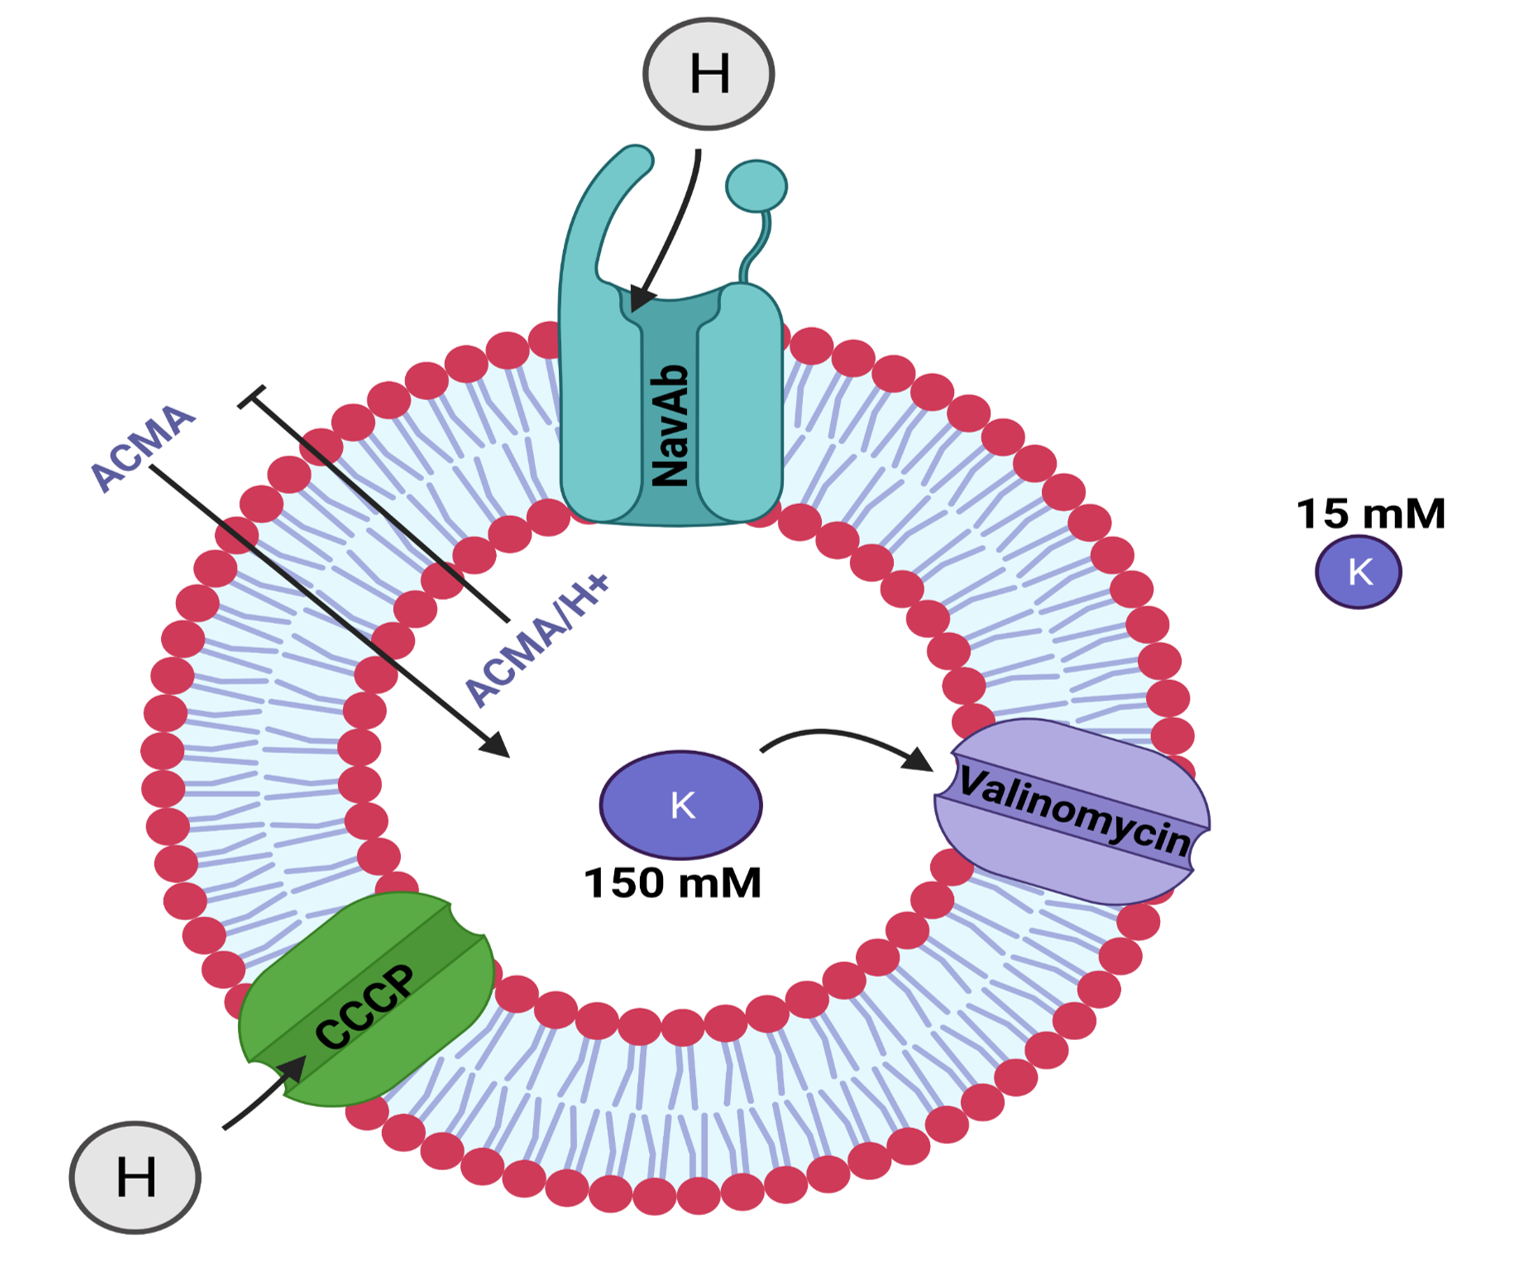
\includegraphics[scale=0.6]{images/picture1.png}}
\caption{\ch{Na+}-insert liposome}
\end{figure}
\end{frame}

\begin{frame}
\label{Practical experimentation}
\frametitle{Practical image of experiment}
\begin{figure}
{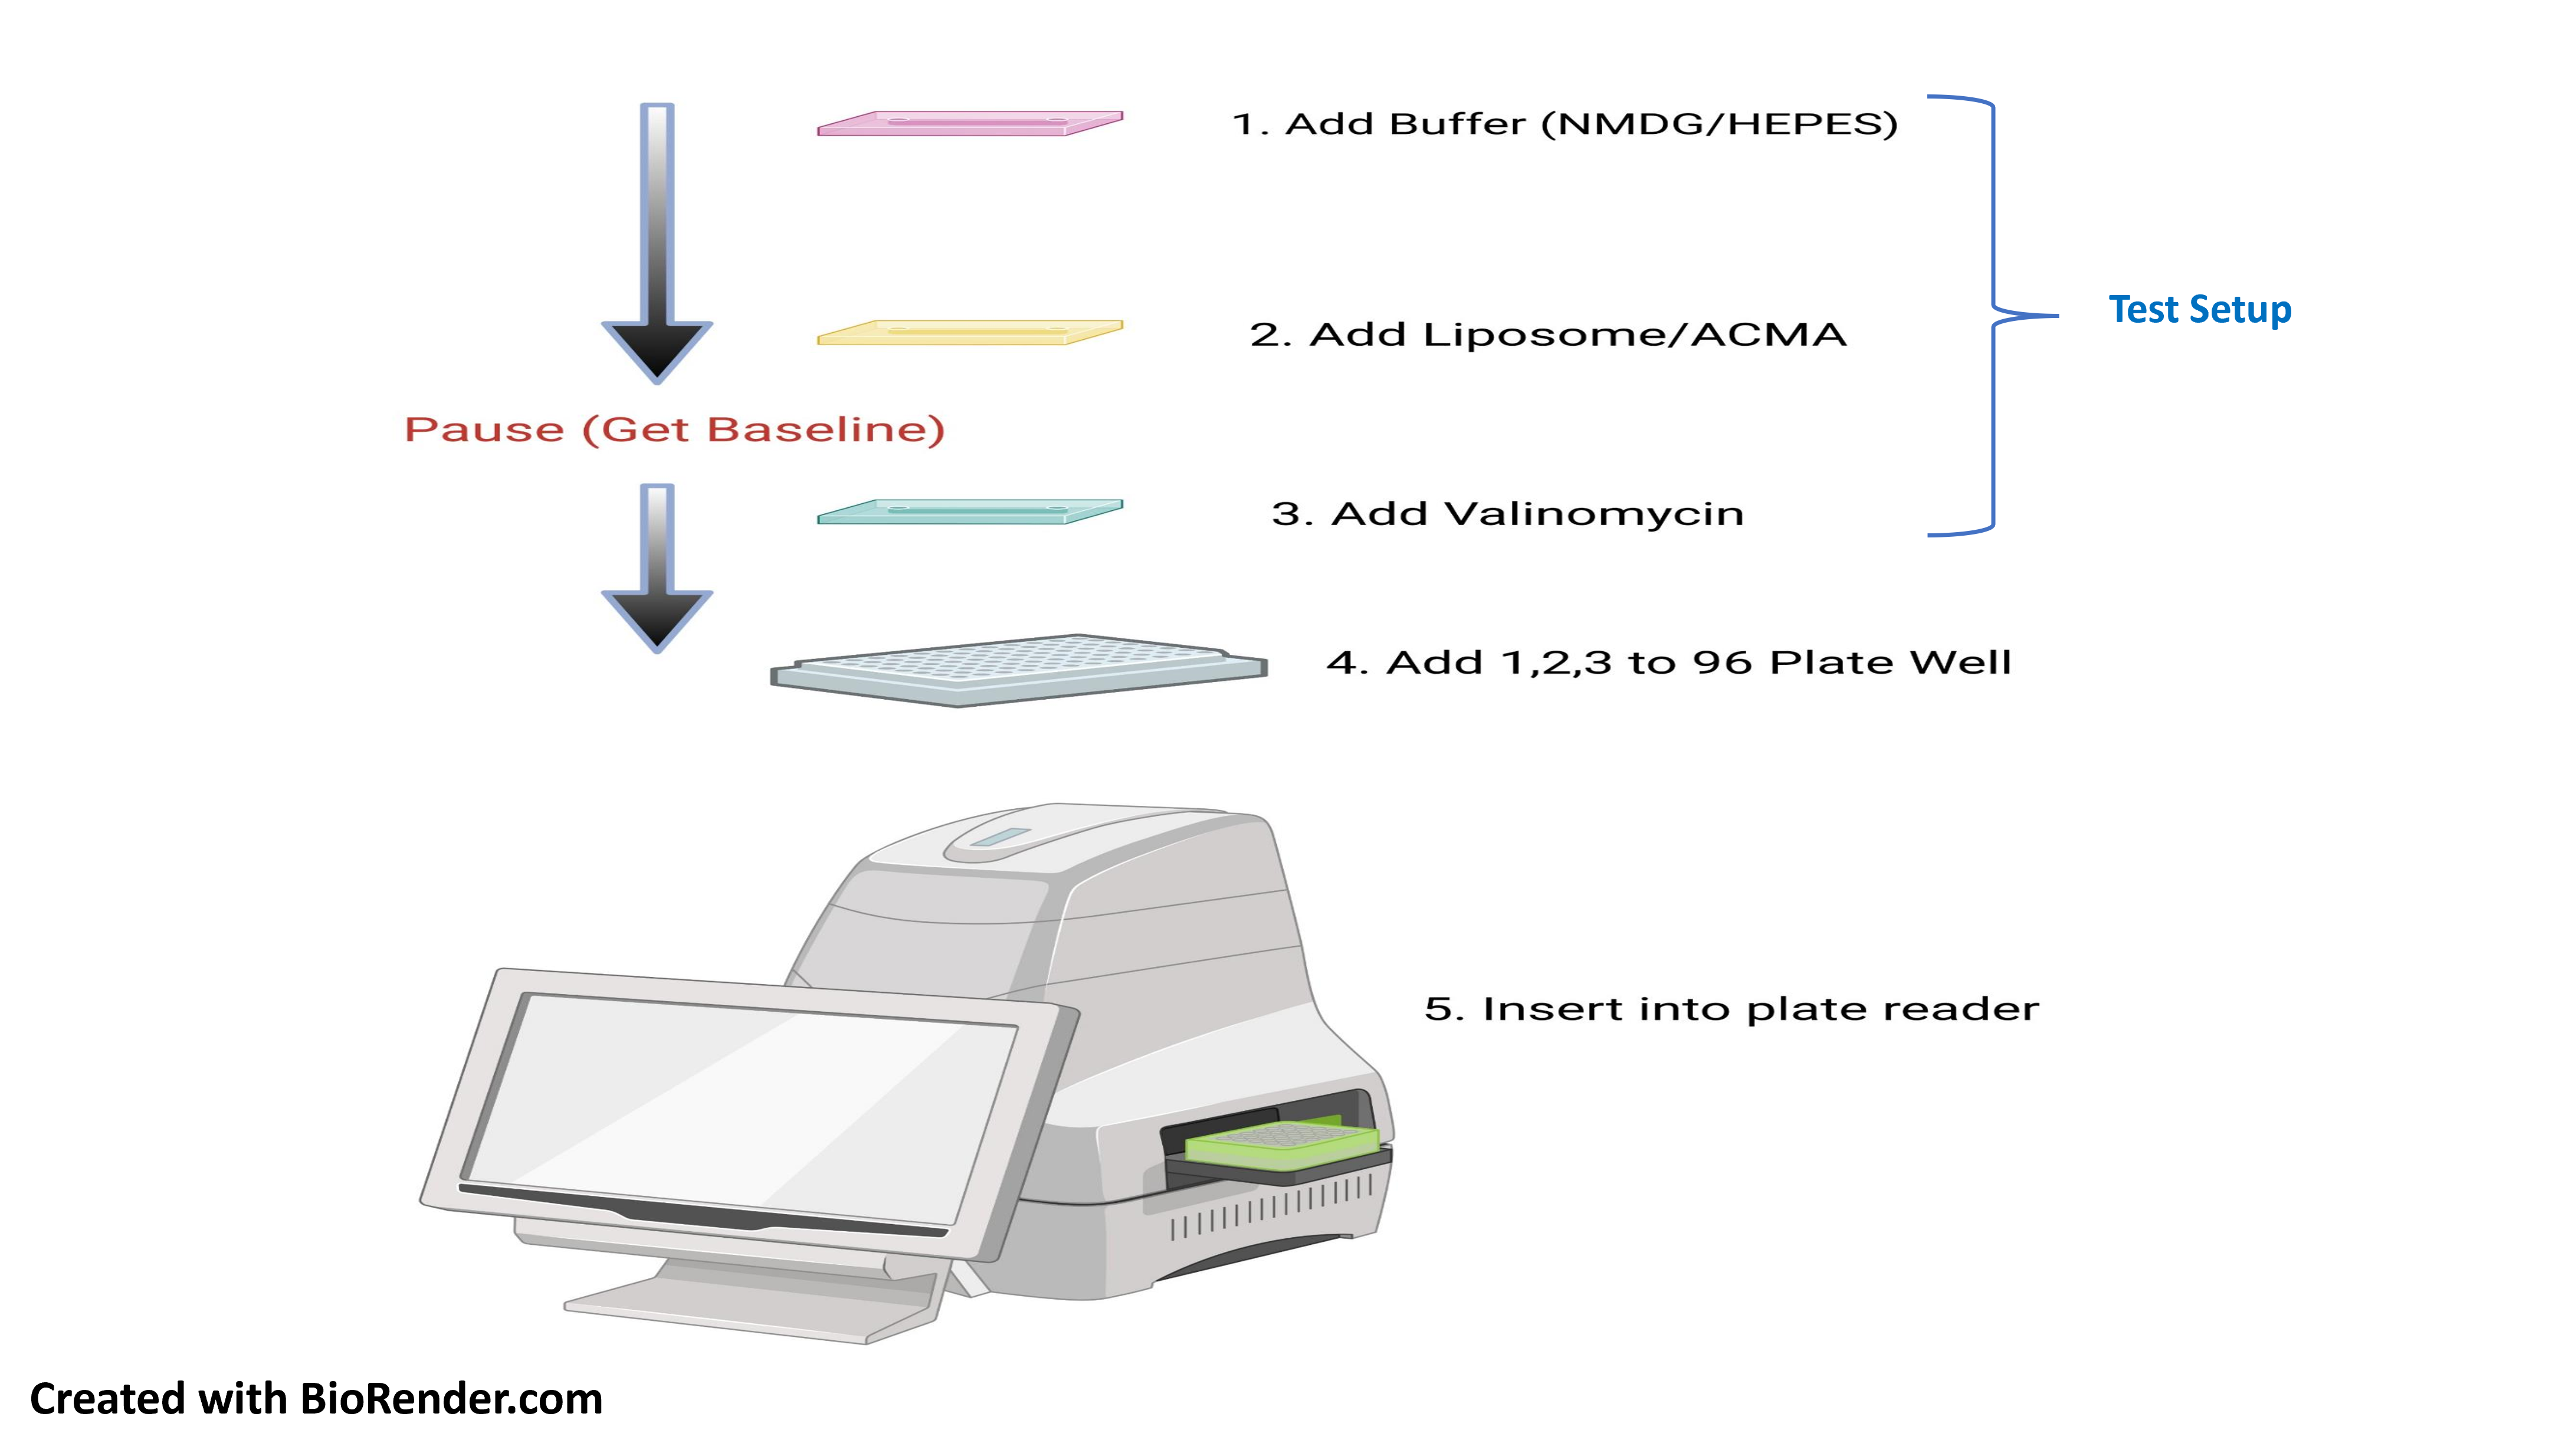
\includegraphics[scale=0.3] {images/picture3.png}}
%{picture3.png}
\caption{experiment}
\end{figure}
\end{frame}


\section{Diagnostic results in Excel}

\subsection{The pitfall of using a sliding scale(Nothing makes sense)}
\begin{frame}
\label{Experimental set-up schematic}
\frametitle{Characteristics of liposome flux assays (LFAs)}
\begin{figure}
{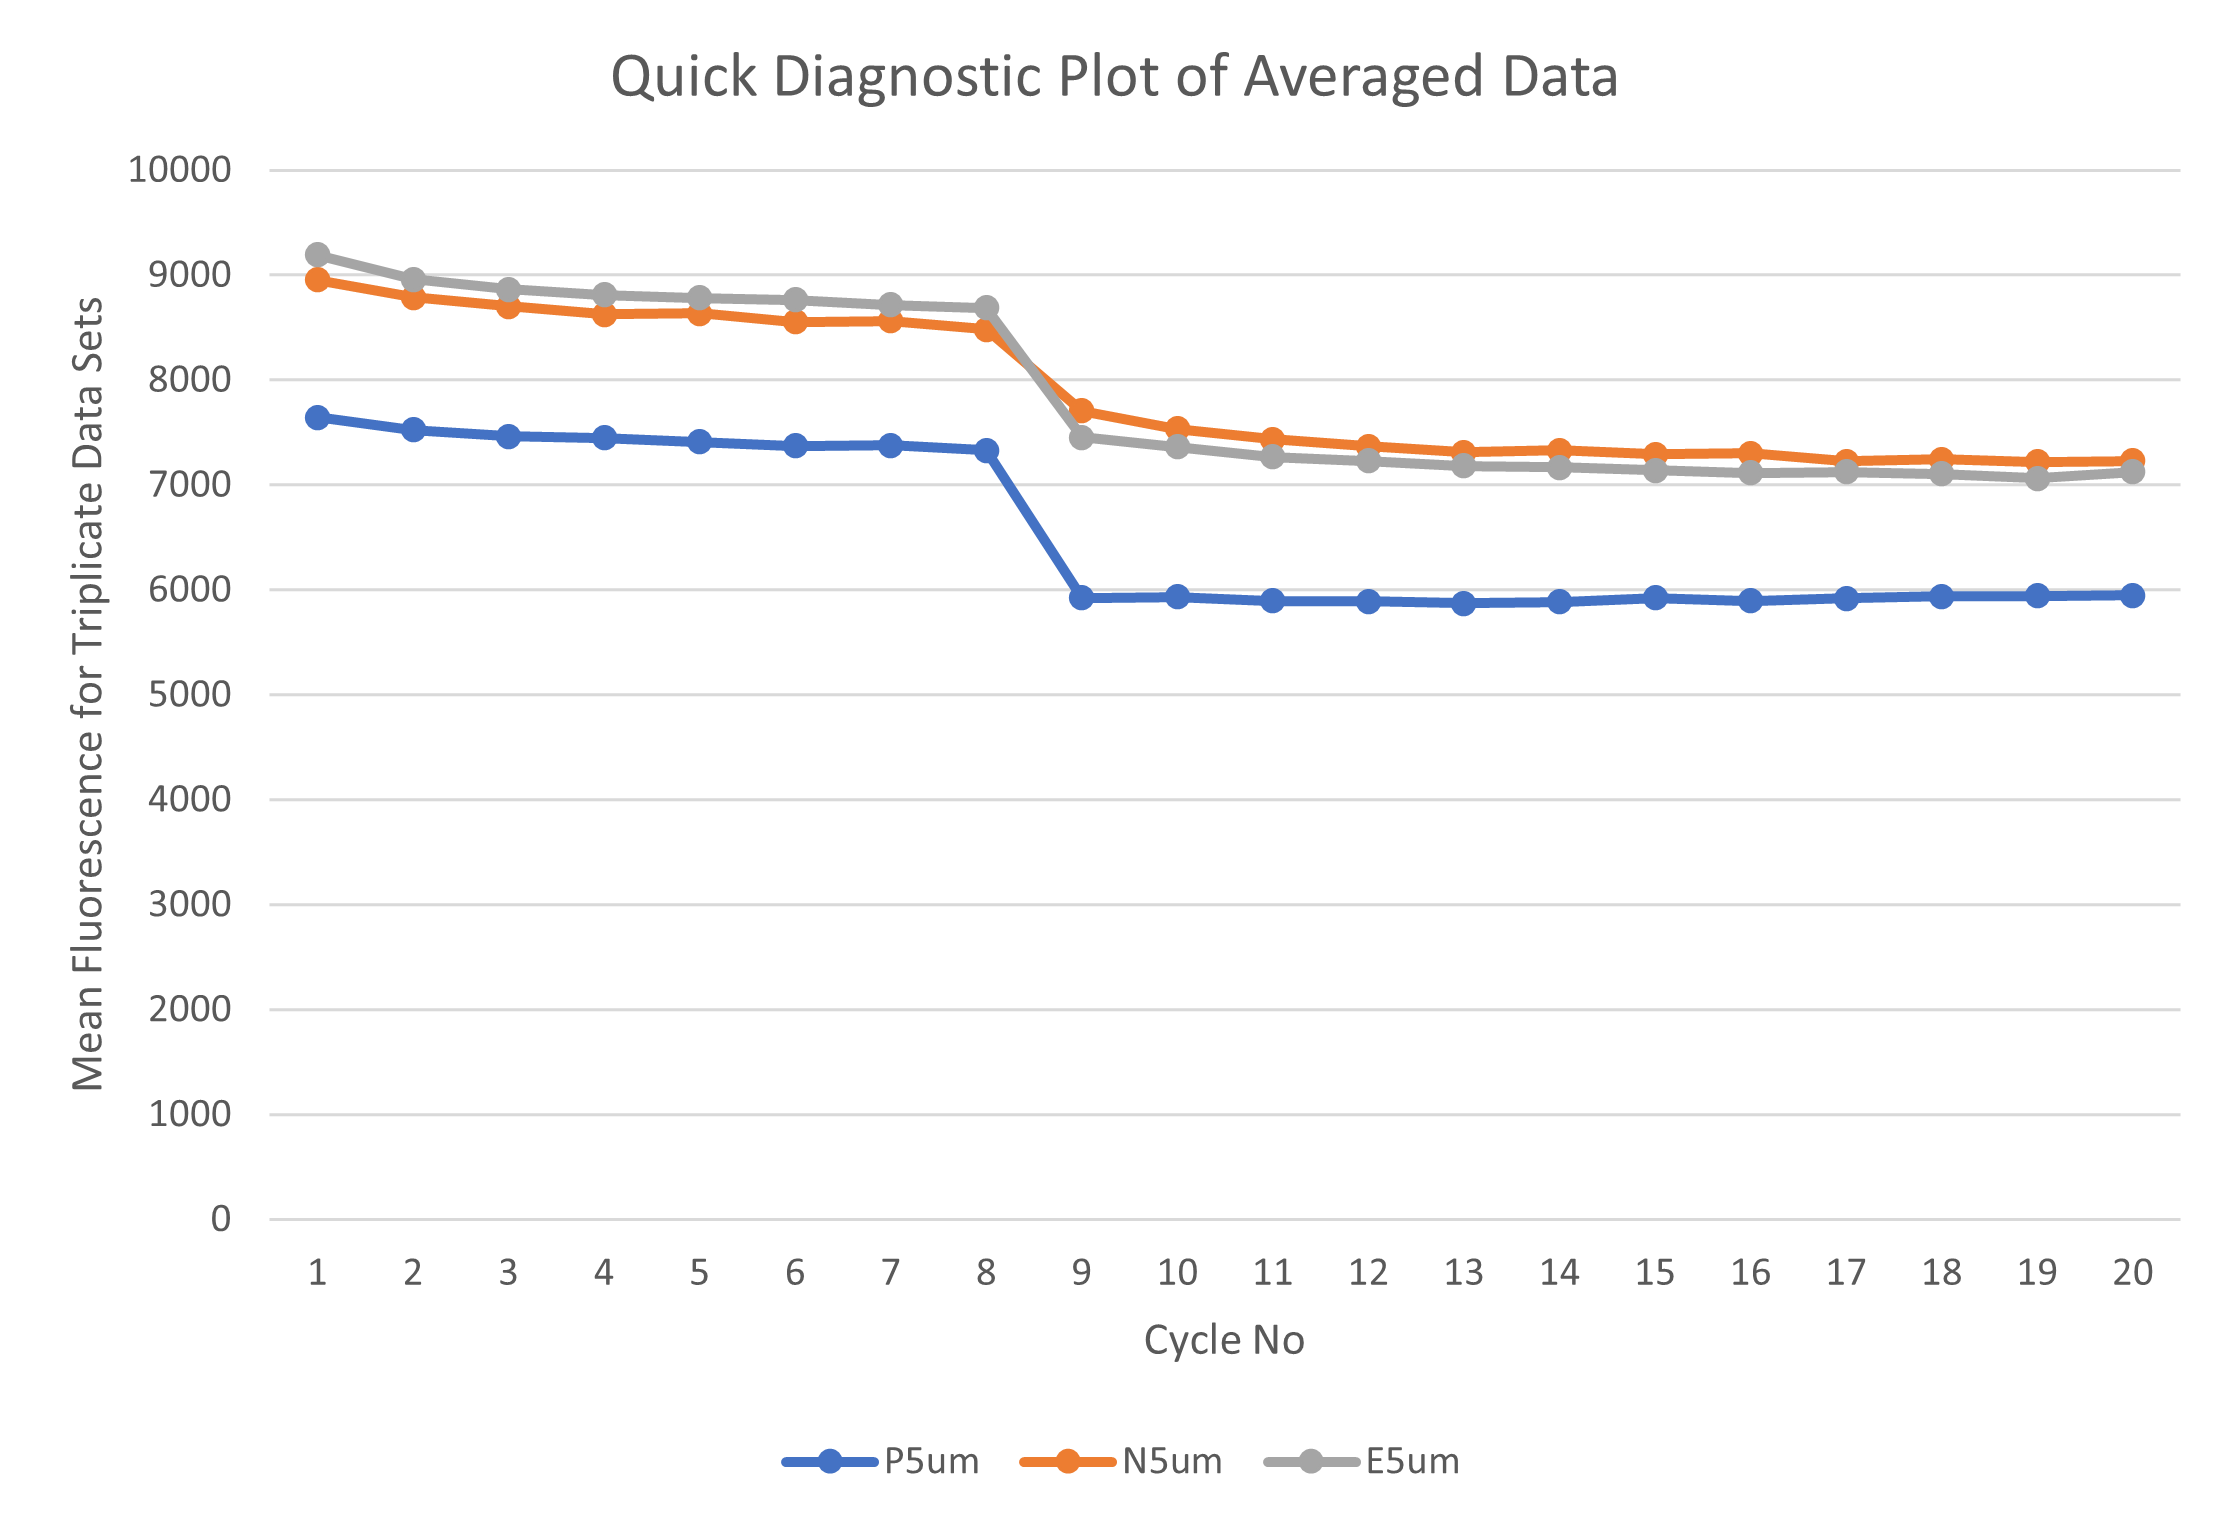
\includegraphics[scale=0.6]{images/picture2.png}}
\caption{\ch{Na+}-insert liposome}
\end{figure}
\end{frame}


\section{Normalized Results (Makes all the sense in the world)}

\subsection{Normalized fluorescence}
\begin{frame}
\label{Fluorescence measured in the signal zone}
\frametitle{Fluorescence measured at 2,3,5 \mu M}
\begin{figure}
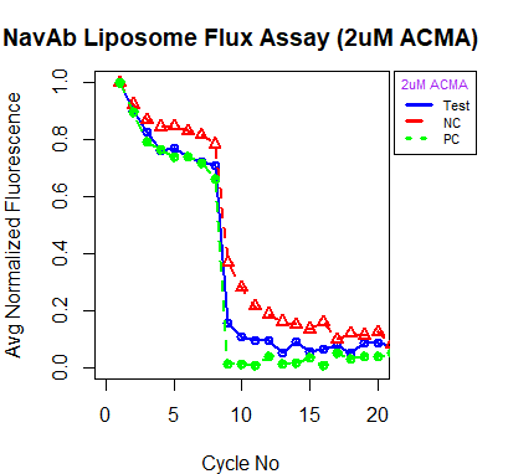
\includegraphics[width=.25\textwidth, valign=t]{images/p6.png}\hfill
    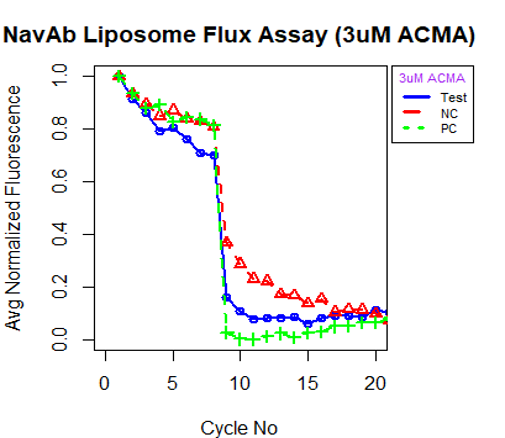
\includegraphics[width=.30\textwidth, valign=t]{images/p5.png}\hfill
     \\[\smallskipamount]
    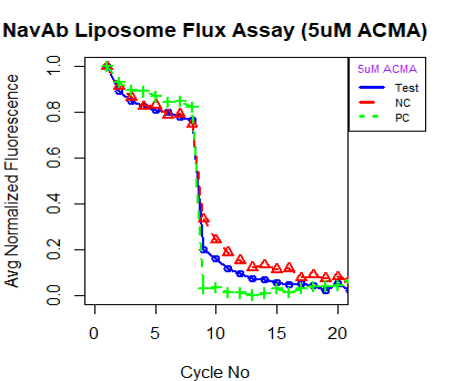
\includegraphics[width=.40\textwidth, valign = c]{images/p4.png}
\caption{Legend: Noramlized fluorescence in R within the signal zone}
\end{figure}
\end{frame}


\subsection{Comparative NavAb conductivity}
\begin{frame}
\label{Comparative NavAb conductivity using Cs and K}
\frametitle{Fluorescence measured with \ch{K+} vs \ch{Cs+} inside the liposome \mu M}
\begin{figure}
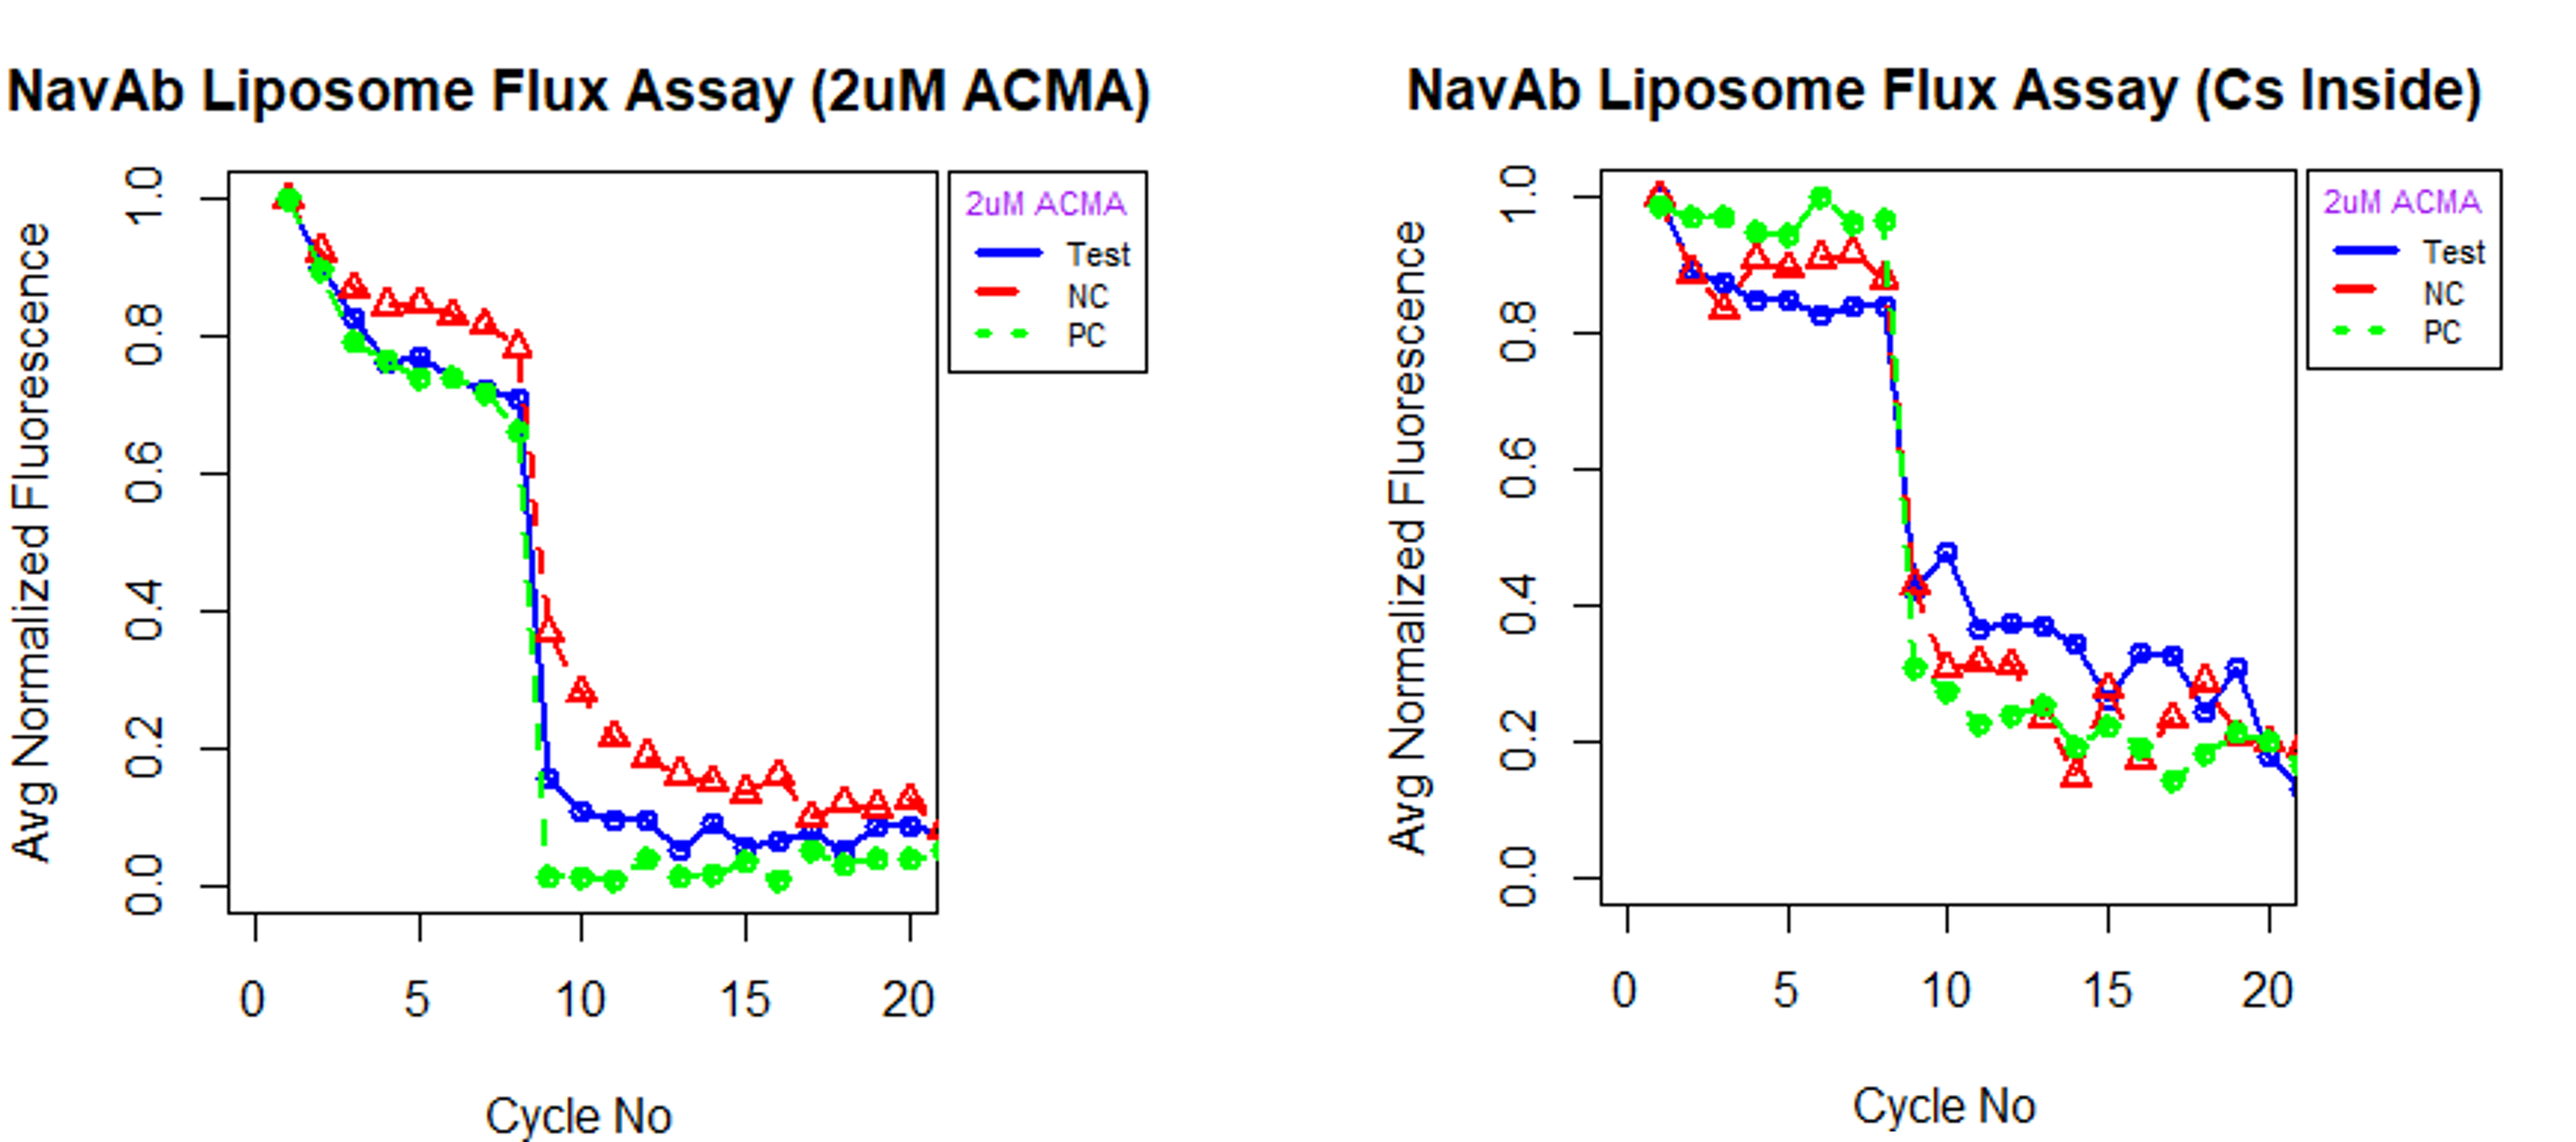
\includegraphics[width=.70\textwidth, valign=t]{images/p7.png}
\caption{NavAb K-conductivity is stronger than Cs-conductivity as indicated by the initial affinity table}
\end{figure}
\end{frame}

\begin{frame}
\label{Comparative NavAb conductivity using Cs and K}
\frametitle{Fluorescence measured with \ch{K+} vs \ch{Cs+} inside the liposome \mu M}
\begin{figure}
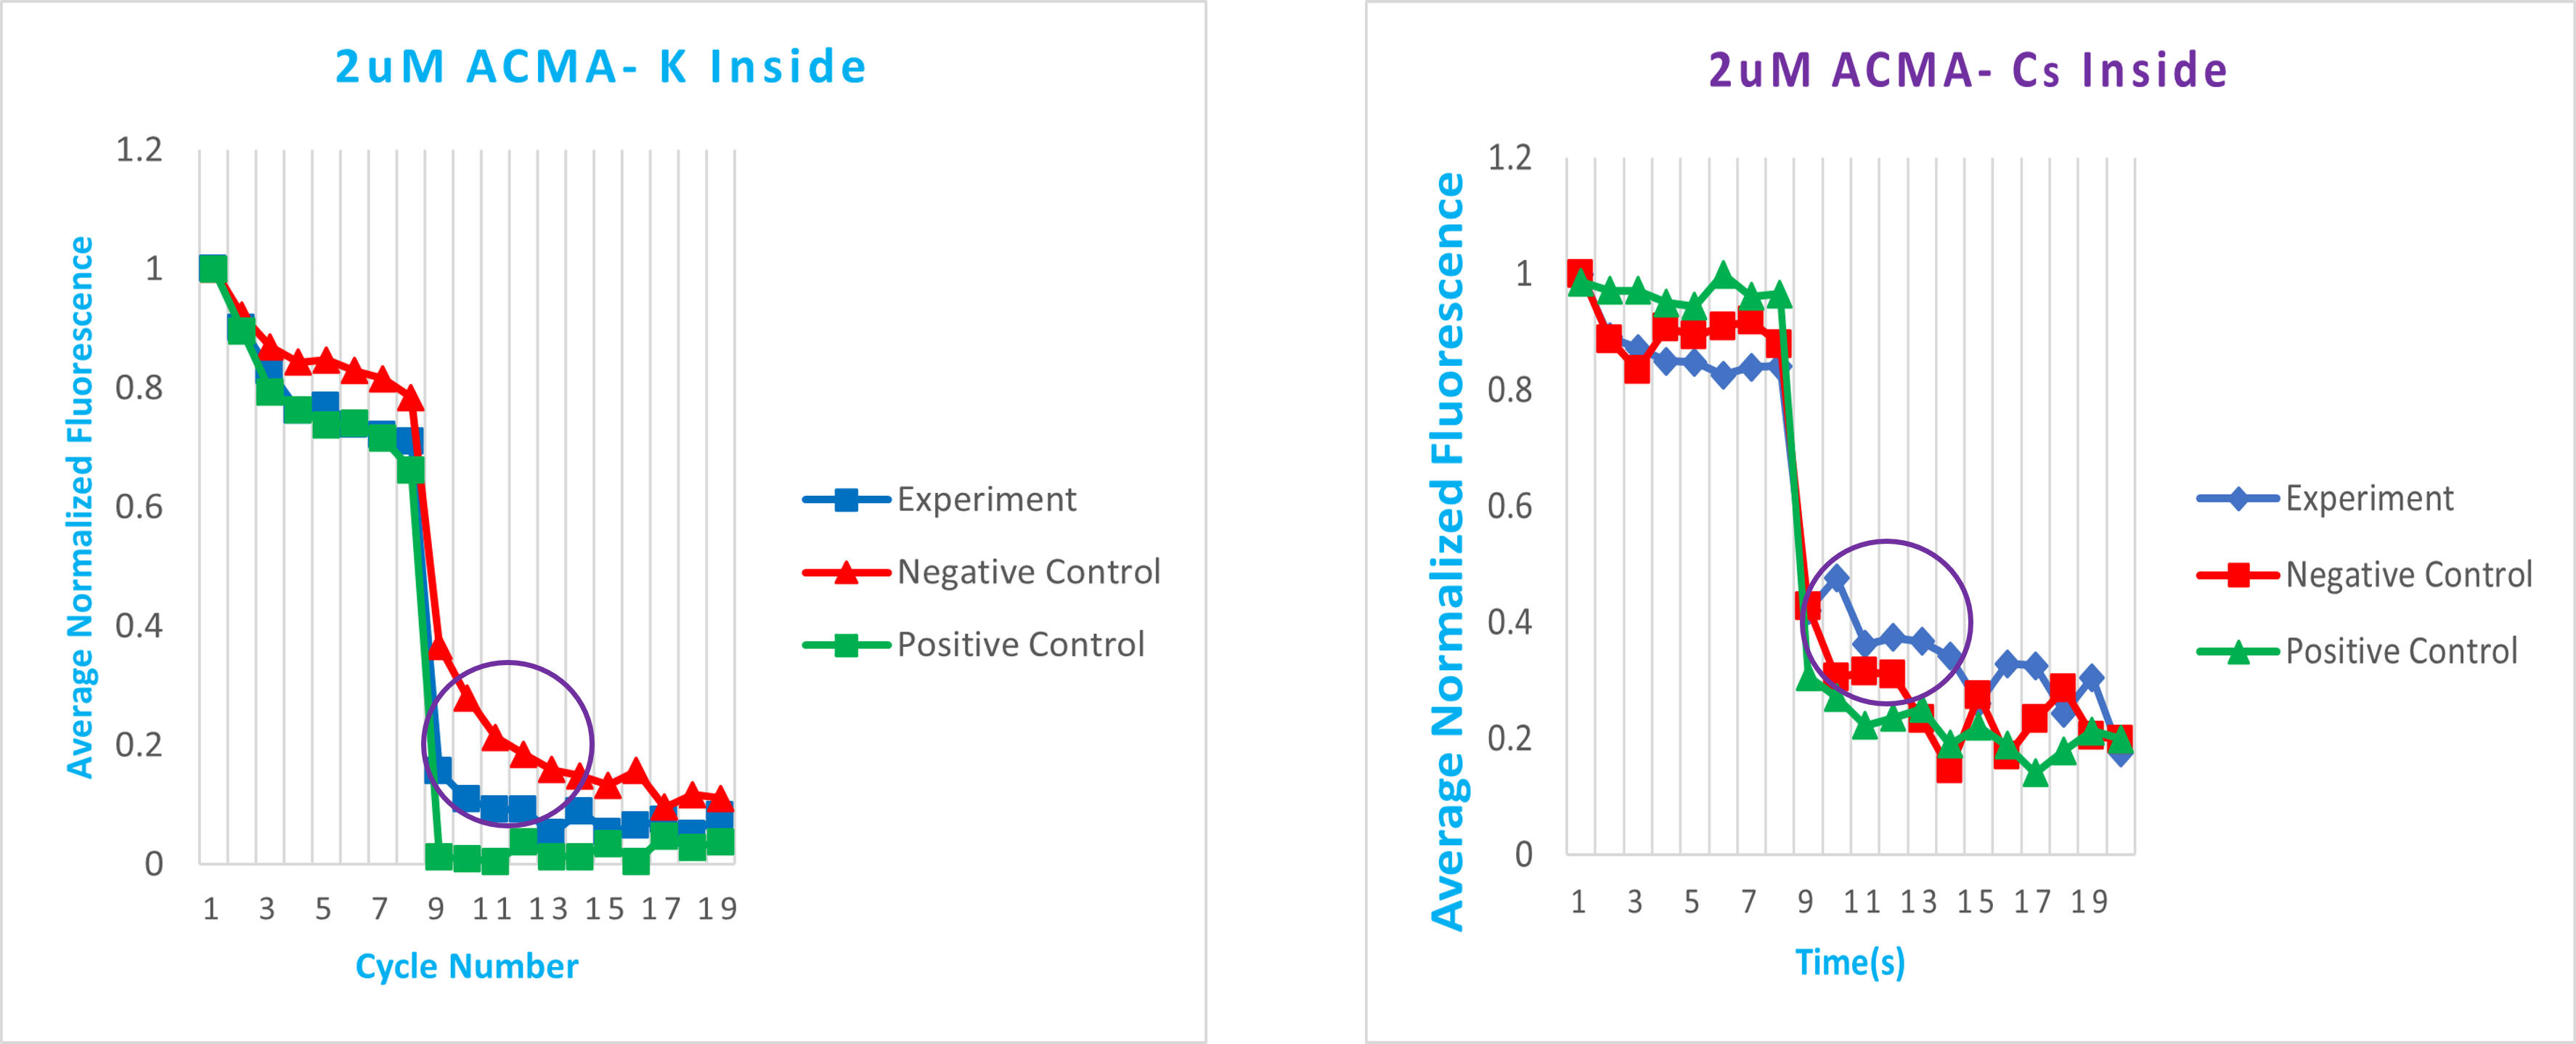
\includegraphics[width=.70\textwidth, valign=t]{images/p8.png}
\caption{NavAb K-conductivity is stronger than Cs-conductivity as indicated by the initial affinity table}
\end{figure}
\end{frame}


\subsection{Fluorophore (ACMA) dosage has no effect on its quenching}
\begin{frame}
\label{ACMA dosage is not important}
\frametitle{ACMA dosage at 2,3,4,5 \mu M}
\begin{figure}
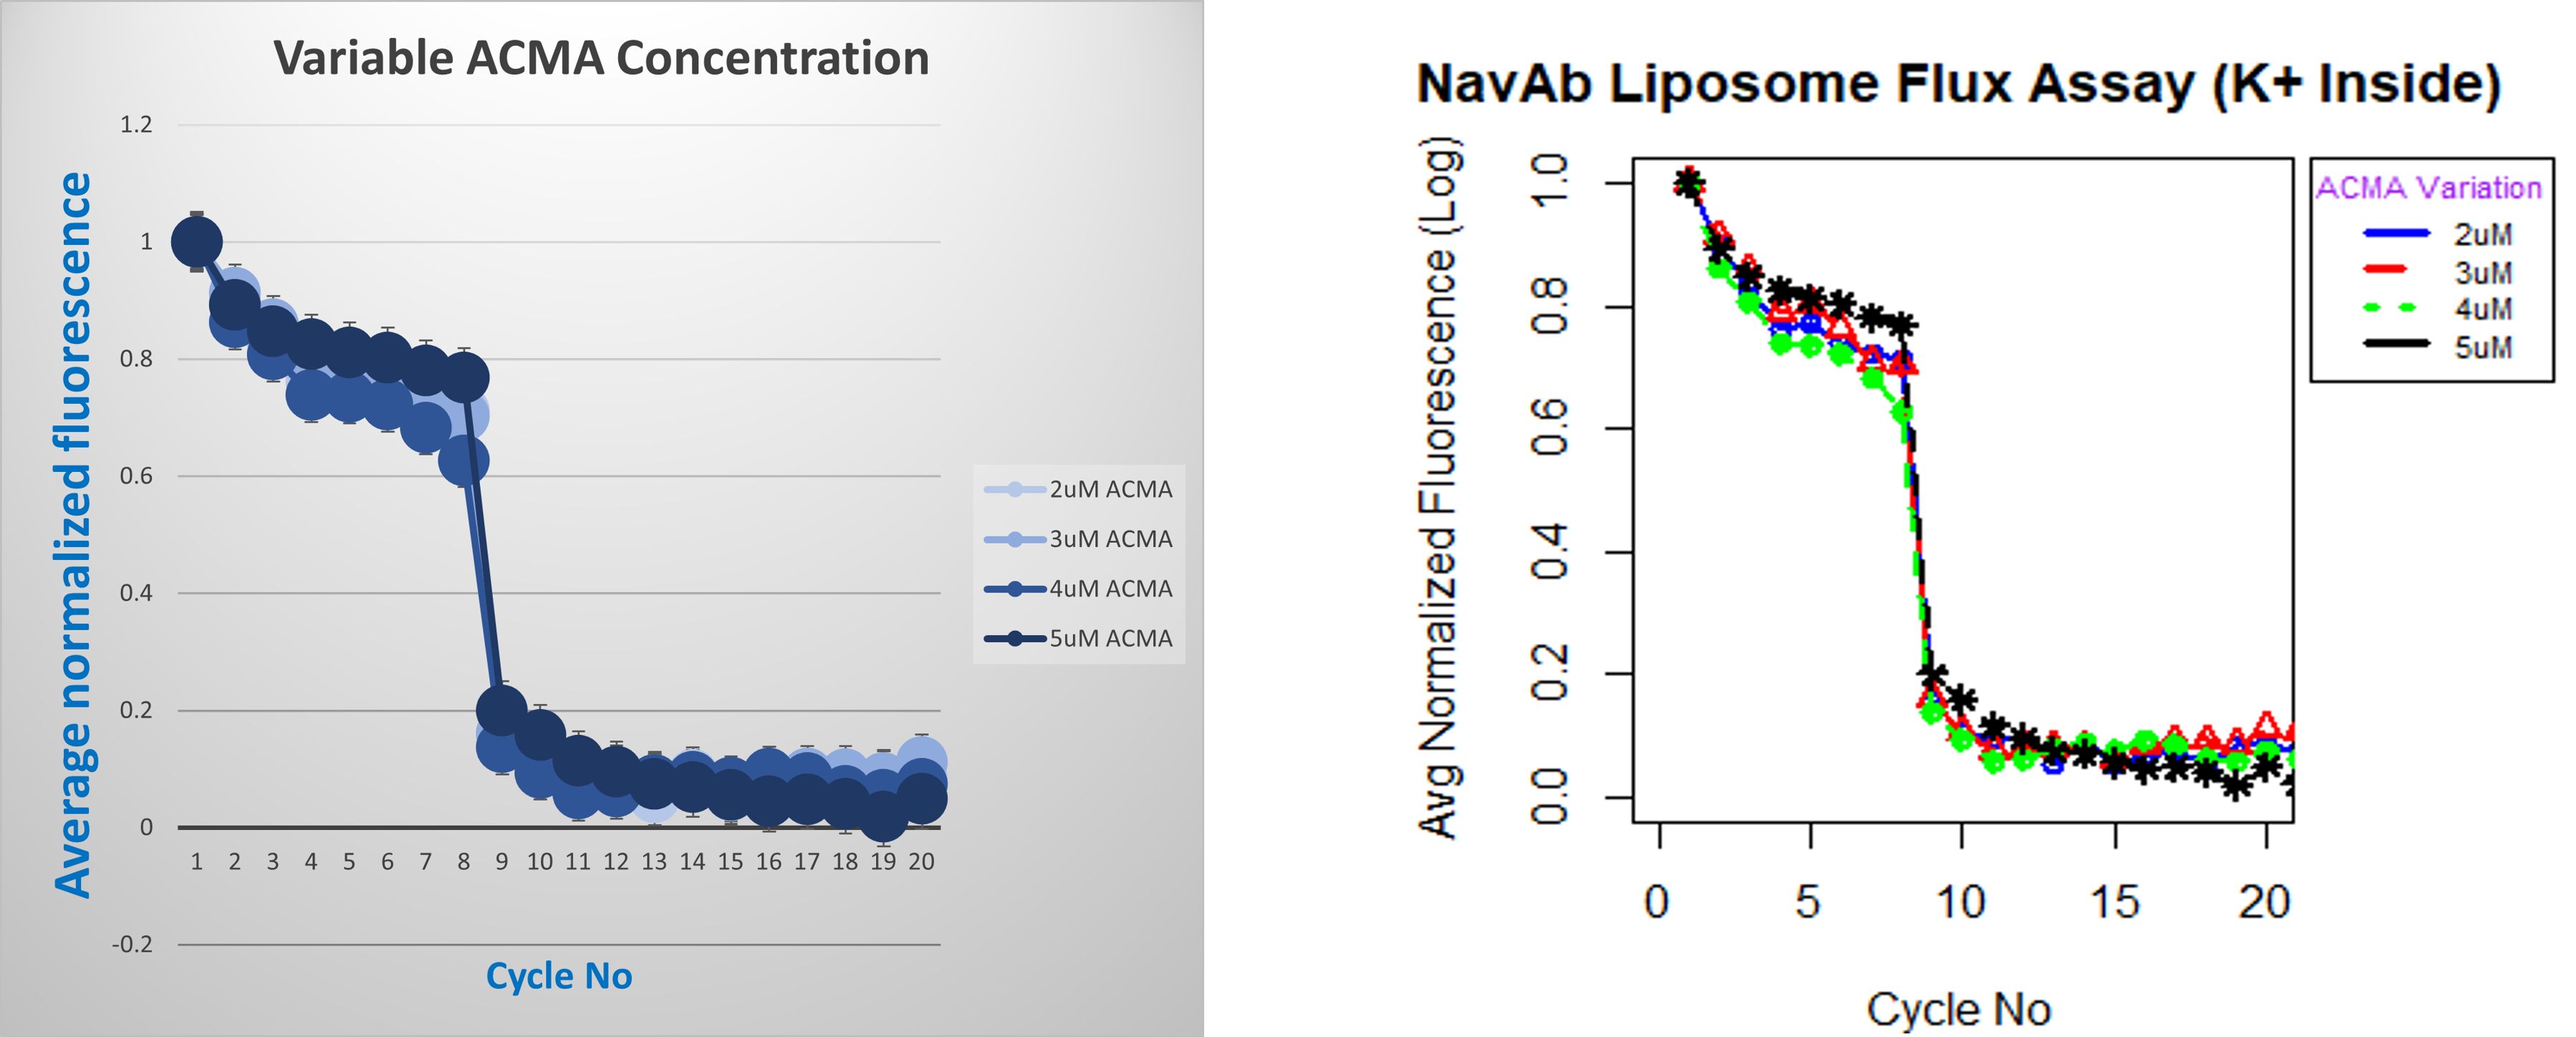
\includegraphics[width=.70\textwidth, valign=t]{images/p9.png}
\caption{Fluorophore dosage is not a factor in its quenching, rather system properties (Ion conductivity etc.) determine quenching}
\end{figure}
\end{frame}

\section{Noise vs Signal}

\subsection{Noise vs Signal is cool}
\begin{frame}
\label{Fluorescence measured in the noise zone}
\frametitle{Fluorescence measured at 0.2 and 20 \mu M}
\begin{figure}
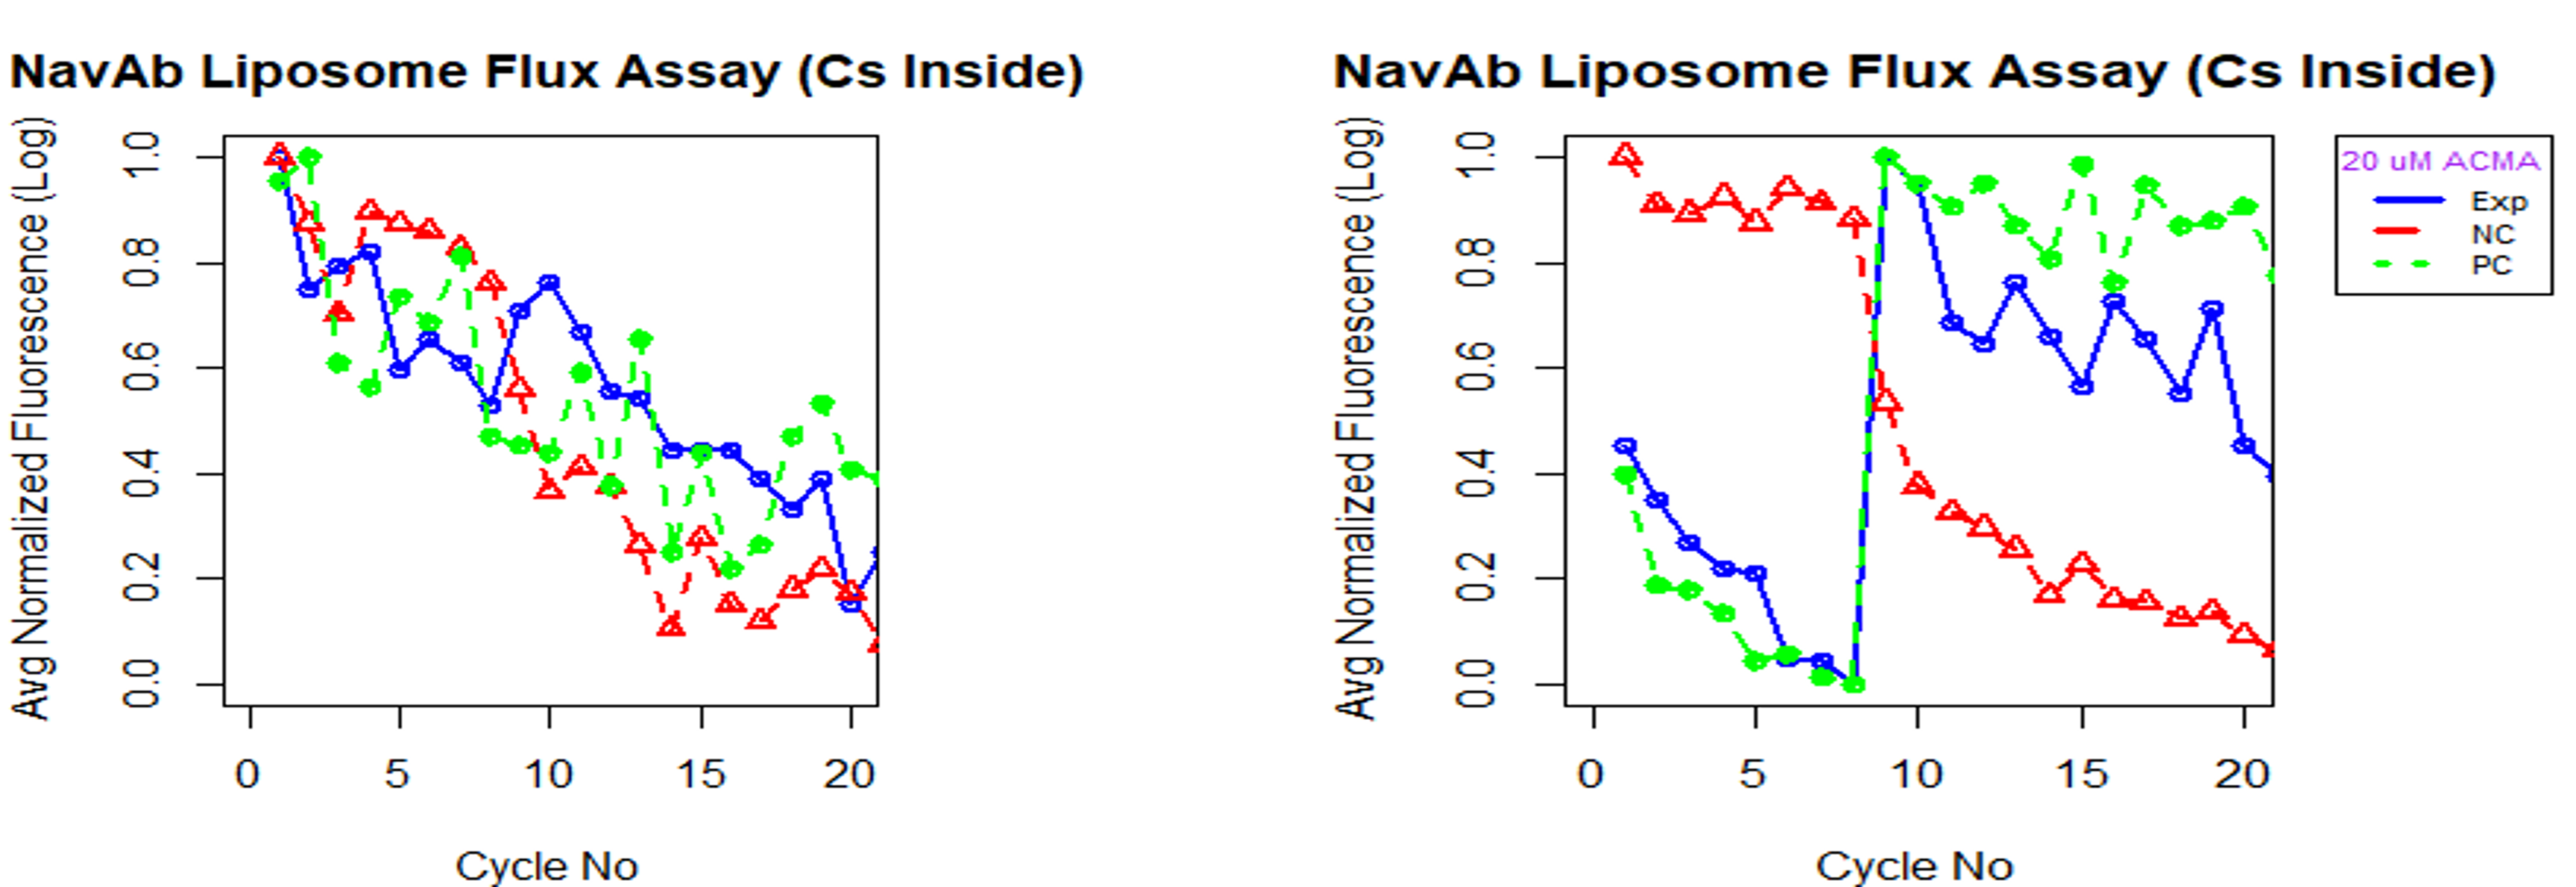
\includegraphics[width=.70\textwidth, valign=t]{images/p10.png}
\caption{Legend: Noramlized fluorescence in R within the signal zone}
\end{figure}
\end{frame}


\section{Conclusion}

\subsection{Conclusions}
 \begin{frame}{Conclusion}
        \begin{block}{Quenching drivers}
            \textbf<2> We showed that the Nernst Potential (Valinomycin) and proton flux (CCCP) should be investigated as potential factors in ACMA quenching behavior. 
        \end{block}
        \pause
        \begin{alertblock}{ACMA concentration}
            \textcolor<6> {orange} We showed that there is a concentration for ACMA to make it useful as a signaling molecule in flux assays.
        \end{alertblock}
        \pause
        \begin{exampleblock}{Noise vs Signal}
            \textcolor<7> {green} We showed that we could use noise to interpret our flux assays.
        \end{exampleblock}
    \end{frame}
    

\begin{frame}[standout]
  \textcolor<7> {orange} Thanks and Questions?
\end{frame}

\appendix

\begin{frame}[standout]{References}

\begin{thebibliography}{1}
\bibitem{su2016} Zhenwi. Su. {\em Novel cell-free high-throughput screening method for pharmacological tools targeting K+ channels.}\/ PNAS,
113(5744-5788), 2016.
\bibitem{su2016} Joshua V. {\em A Single Molecule Study on The Structural Basis of Ion Selective Permeation in Voltage-Gated Sodium Channels.}\/ , 2021.
\end{thebibliography}

\end{frame}


\end{document}
